\section{eo\-How\-Many Class Reference}
\label{classeo_how_many}\index{eoHowMany@{eoHowMany}}
A helper class, to determine a number of individuals from another one Typically, is used in selection / replacement procedures, e.g.  


{\tt \#include $<$eo\-How\-Many.h$>$}

Inheritance diagram for eo\-How\-Many::\begin{figure}[H]
\begin{center}
\leavevmode
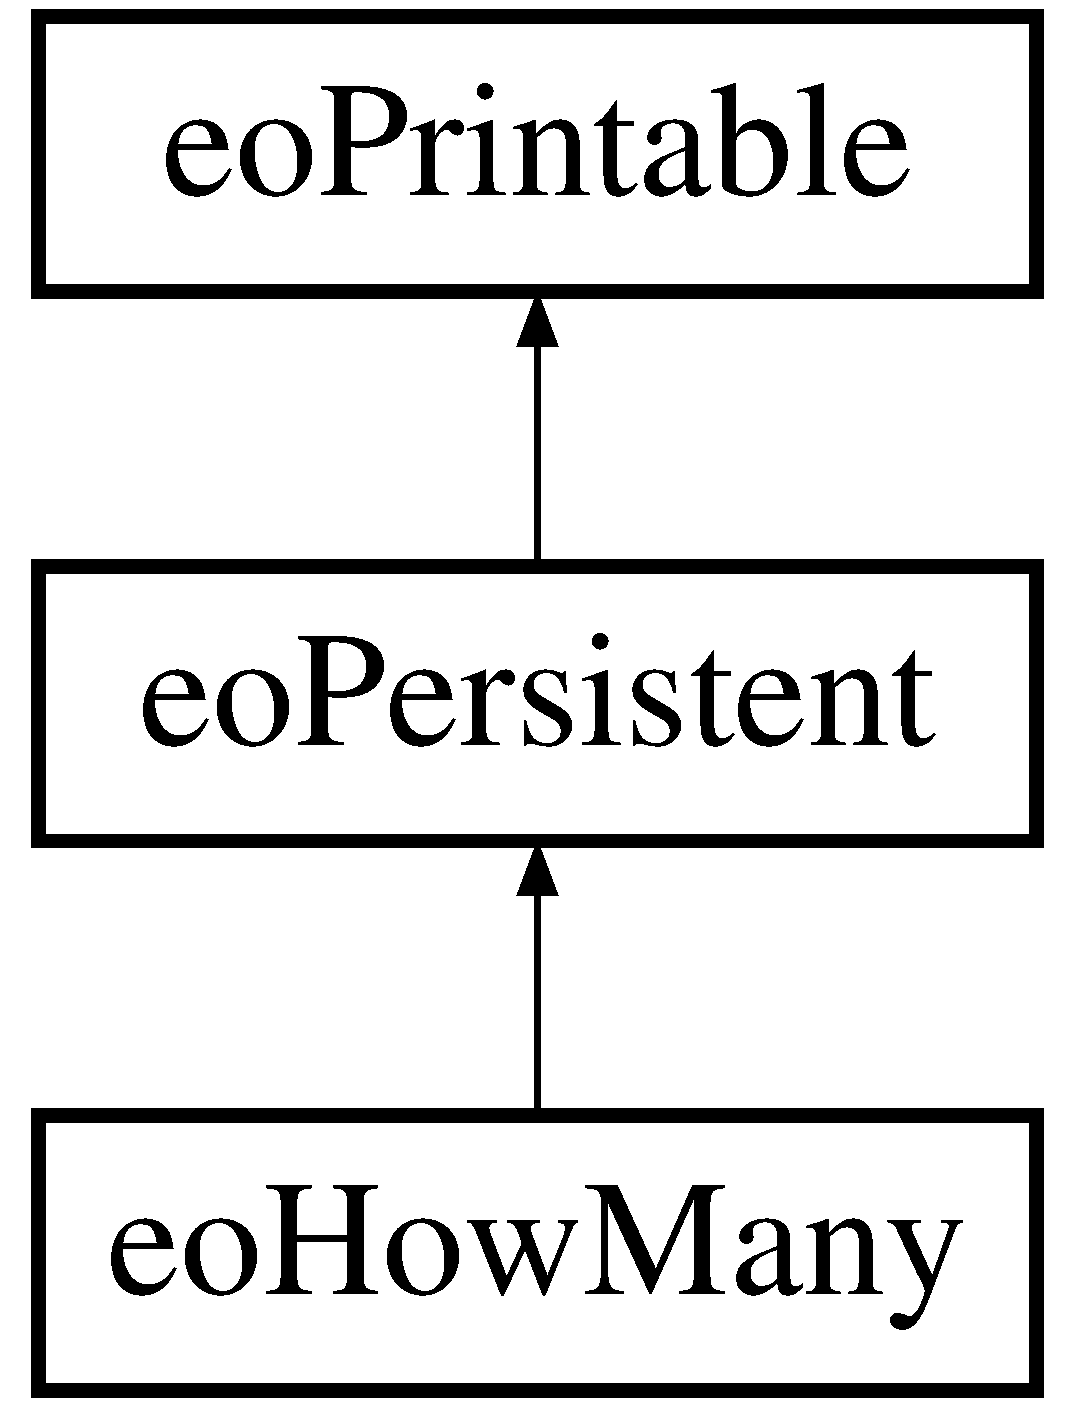
\includegraphics[height=3cm]{classeo_how_many}
\end{center}
\end{figure}
\subsection*{Public Member Functions}
\begin{CompactItemize}
\item 
{\bf eo\-How\-Many} (double \_\-rate=0.0, bool \_\-interpret\_\-as\_\-rate=true)
\begin{CompactList}\small\item\em Original Ctor from direct rate + bool. \item\end{CompactList}\item 
{\bf eo\-How\-Many} (int \_\-combien)\label{classeo_how_many_a1}

\begin{CompactList}\small\item\em Ctor from an int - both from int and unsigned int are needed to avoid ambiguity with the Ctor from a double. \item\end{CompactList}\item 
{\bf eo\-How\-Many} (unsigned int \_\-combien)\label{classeo_how_many_a2}

\begin{CompactList}\small\item\em Ctor from an unsigned int - both from int and unsigned int are needed to avoid ambiguity with the Ctor from a double. \item\end{CompactList}\item 
virtual {\bf $\sim$eo\-How\-Many} ()\label{classeo_how_many_a3}

\begin{CompactList}\small\item\em Virtual dtor. They are needed in virtual class hierarchies. \item\end{CompactList}\item 
unsigned int {\bf operator()} (unsigned int \_\-size)
\begin{CompactList}\small\item\em Does what it was designed for combien==0 : return rate$\ast$\_\-size else combien$>$0 : return combien (regardless of \_\-size) combien$<$0 : return \_\-size-$|$combien$|$. \item\end{CompactList}\item 
virtual void {\bf print\-On} (std::ostream \&\_\-os) const 
\begin{CompactList}\small\item\em Write object. \item\end{CompactList}\item 
virtual void {\bf read\-From} (std::istream \&\_\-is)
\begin{CompactList}\small\item\em Read object. \item\end{CompactList}\item 
void {\bf read\-From} (std::string \_\-value)\label{classeo_how_many_a7}

\item 
{\bf eo\-How\-Many} {\bf operator-} ()\label{classeo_how_many_a8}

\begin{CompactList}\small\item\em The unary - operator: reverses the computation. \item\end{CompactList}\end{CompactItemize}
\subsection*{Private Attributes}
\begin{CompactItemize}
\item 
double {\bf rate}\label{classeo_how_many_r0}

\item 
int {\bf combien}\label{classeo_how_many_r1}

\end{CompactItemize}


\subsection{Detailed Description}
A helper class, to determine a number of individuals from another one Typically, is used in selection / replacement procedures, e.g. 

the number of offspring from the number of parents, or the number of survivors for an {\bf eo\-Reduce}{\rm (p.\,\pageref{classeo_reduce})} functor, ...

Such construct is very useful because in some cases you might not know the population size that will enter the replacement. For instance, you cannot simply have a pre-computed (double) rate of 1/pop\-Size if you want to select or kill just 1 guy. Using an eo\-How\-Many allows one to modify the population size without touching anything else.

There are 4 possible way to compute the return value from the argument:\begin{itemize}
\item an absolute POSITIVE integer --$>$ return it (regardless of popsize)\item a POSITIVE rate --$>$ return rate$\ast$pop\-Size\item an absolute NEGATIVE integer --$>$ return popsize-rate (if positive)\item a NEGATIVE rate in [-1,0] --$>$ store and use 1-$|$rate$|$ (positive) Note that a negative rate should be have been necessary because a rate is relative, but it is there for consistency reasons - and because it is needed in {\tt eo\-G3Replacement}\end{itemize}


It has 2 private members, a double and an integer to cover all cases

Example use: in {\tt eo\-General\-Breeder.h} Example reading from parser: in {\tt do/make\_\-algo\_\-scalar.h line 141}

MS 10/04/2002: Added the possibility to have a negative number - when treated as a number: returns then (size - combien) Should not modify anything when a positive number is passed in the ctor

MS 20/06/2002: Added the negative rate and the {\bf operator-()}{\rm (p.\,\pageref{classeo_how_many_a8})} (for eo\-G3Repalcement)

It is an {\bf eo\-Persistent}{\rm (p.\,\pageref{classeo_persistent})} because we need to be able to use eo\-Param\-Value$<$eo\-How\-Many$>$ 



Definition at line 69 of file eo\-How\-Many.h.

\subsection{Constructor \& Destructor Documentation}
\index{eoHowMany@{eo\-How\-Many}!eoHowMany@{eoHowMany}}
\index{eoHowMany@{eoHowMany}!eoHowMany@{eo\-How\-Many}}
\subsubsection{\setlength{\rightskip}{0pt plus 5cm}eo\-How\-Many::eo\-How\-Many (double {\em \_\-rate} = {\tt 0.0}, bool {\em \_\-interpret\_\-as\_\-rate} = {\tt true})\hspace{0.3cm}{\tt  [inline]}}\label{classeo_how_many_a0}


Original Ctor from direct rate + bool. 

\begin{Desc}
\item[Parameters:]
\begin{description}
\item[{\em rate}]the rate, OR the integer to store, depending on 2nd arg. \item[{\em \_\-interpret\_\-as\_\-rate}]to tell whether the rate actually is a rate \end{description}
\end{Desc}


Definition at line 76 of file eo\-How\-Many.h.

\subsection{Member Function Documentation}
\index{eoHowMany@{eo\-How\-Many}!operator()@{operator()}}
\index{operator()@{operator()}!eoHowMany@{eo\-How\-Many}}
\subsubsection{\setlength{\rightskip}{0pt plus 5cm}unsigned int eo\-How\-Many::operator() (unsigned int {\em \_\-size})\hspace{0.3cm}{\tt  [inline]}}\label{classeo_how_many_a4}


Does what it was designed for combien==0 : return rate$\ast$\_\-size else combien$>$0 : return combien (regardless of \_\-size) combien$<$0 : return \_\-size-$|$combien$|$. 

\begin{itemize}
\item $\ast$ - $\ast$ - $\ast$ - \end{itemize}


Definition at line 114 of file eo\-How\-Many.h.\index{eoHowMany@{eo\-How\-Many}!printOn@{printOn}}
\index{printOn@{printOn}!eoHowMany@{eo\-How\-Many}}
\subsubsection{\setlength{\rightskip}{0pt plus 5cm}virtual void eo\-How\-Many::print\-On (std::ostream \& {\em \_\-os}) const\hspace{0.3cm}{\tt  [inline, virtual]}}\label{classeo_how_many_a5}


Write object. 

It's called print\-On since it prints the object on a stream. \begin{Desc}
\item[Parameters:]
\begin{description}
\item[{\em \_\-os}]A std::ostream. \end{description}
\end{Desc}


Implements {\bf eo\-Printable} {\rm (p.\,\pageref{classeo_printable_a1})}.

Definition at line 130 of file eo\-How\-Many.h.\index{eoHowMany@{eo\-How\-Many}!readFrom@{readFrom}}
\index{readFrom@{readFrom}!eoHowMany@{eo\-How\-Many}}
\subsubsection{\setlength{\rightskip}{0pt plus 5cm}virtual void eo\-How\-Many::read\-From (std::istream \& {\em \_\-is})\hspace{0.3cm}{\tt  [inline, virtual]}}\label{classeo_how_many_a6}


Read object. 

\begin{Desc}
\item[Parameters:]
\begin{description}
\item[{\em \_\-is}]A std::istream. \end{description}
\end{Desc}
\begin{Desc}
\item[Exceptions:]
\begin{description}
\item[{\em runtime\_\-std::exception}]If a valid object can't be read. \end{description}
\end{Desc}


Implements {\bf eo\-Persistent} {\rm (p.\,\pageref{classeo_persistent_a1})}.

Definition at line 140 of file eo\-How\-Many.h.

The documentation for this class was generated from the following file:\begin{CompactItemize}
\item 
eo\-How\-Many.h\end{CompactItemize}
